\subsection{Results for Trajectories Estimated Using $x$ and $y$ Offset}
%\label{subsec:no_abs_results}
%\vspace{10pt}

Figure~\ref{fig:var_no abs.png} represents the $p$-values for the Mann-Whitney $U$-test on actual and predicted values across k-fold validation datasets for the trajectories estimated using $x$ and $y$ offset in the k-fold testing datasets using different RNN models, and forecasting times. Darker colors in grayscale represent a higher $p$-value in a range from $0$ to $1$. The values on the secondary diagonal are all equal to $1$ and black beacuse each model is equal to itself.

\begin{figure}[!ht]
	\centering
	\includegraphics[width = 0.99 \linewidth]{var_no abs.png.pdf}
	\caption{The $p$-values for the Mann-Whitney $U$-test on actual and predicted values across k-fold validation datasets for the trajectories estimated using $x$ and $y$ offset in the k-fold testing datasets using different RNN models, and forecasting times. Darker colors in grayscale represent a higher $p$-value in a range from $0$ to $1$. The values on the secondary diagonal are all equal to $1$ and black beacuse each model is equal to itself.}
	\label{fig:var_no abs.png}
\end{figure}

Figure~\ref{fig:best_R2_traj_val} contains the average $R^{2}$ (\%) across k-fold testing datasets using different trajectory estimation methods, validation datasets for all trajectories estimated in nested k-fold cross-validation by different trajectory estimation methods, RNN models, and forecasting times.

\begin{figure}[!ht]
	\centering
	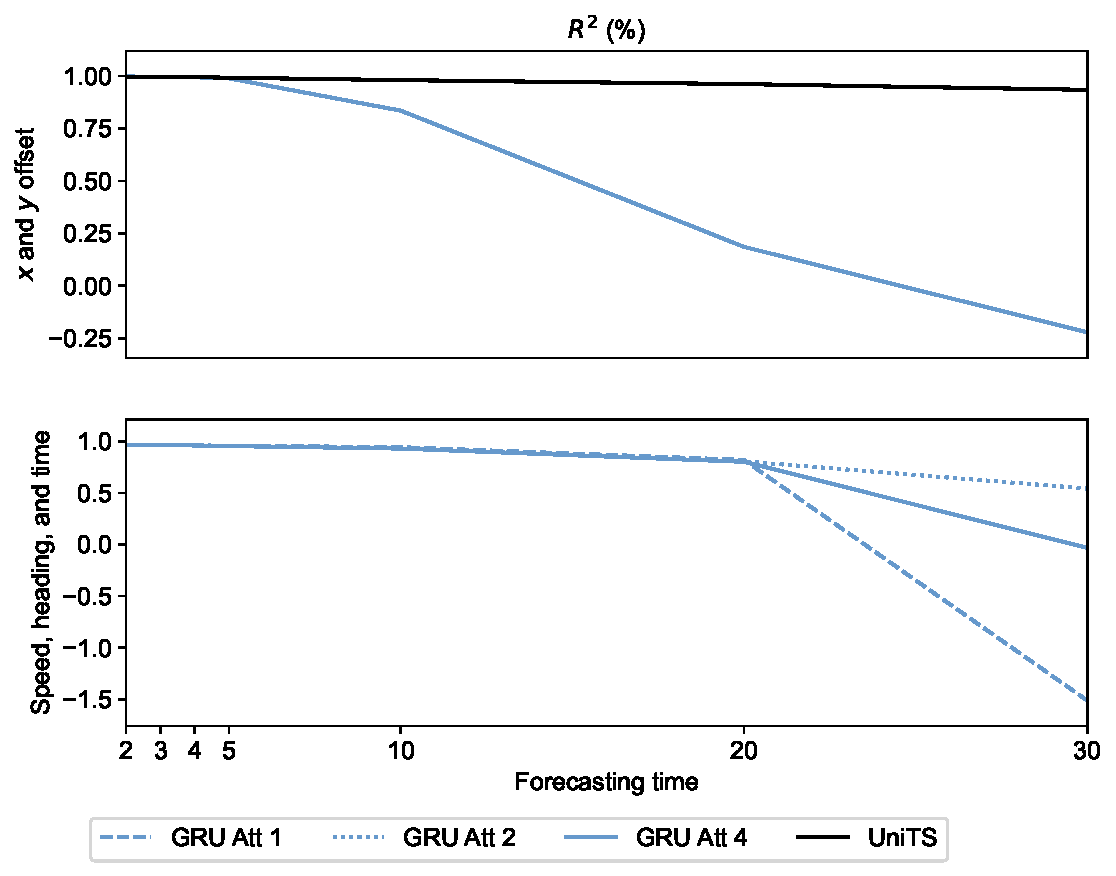
\includegraphics[width = 0.99 \linewidth]{best_R2_traj_val.pdf}
	\caption{The average $R^{2}$ (\%) across k-fold testing datasets using different trajectory estimation methods, validation datasets for all trajectories estimated in nested k-fold cross-validation by different trajectory estimation methods, RNN models, and forecasting times.}
	\label{fig:best_R2_traj_val}
\end{figure}

The average $R^{2}$ (\%), with standard deviation in brackets, across k-fold validation datasets for the trajectories in the k-fold testing datasets estimated using $x$ and $y$ offset, different RNN models, and forecasting times is listed in Table~\ref{tab:best_no_abs_R2}.

\begin{table}[!ht]
	\centering
	\resizebox{\linewidth}{!}{
		\begin{tabular}{|c|c|c|c|c|c|c|c|}
			\hline
			Model & $2$ $s$ & $3$ $s$ & $4$ $s$ & $5$ $s$ & $10$ $s$ & $20$ $s$ & $30$ $s$ \\ \hline
			\multirow{2}{*}{GRU Att 4} & $\mathbf{99.75\%}$ & $\mathbf{99.59\%}$ & $99.38\%$ & $98.86\%$ & $83.46\%$ & $18.51\%$ & $-22.18\%$ \\
			 & \textbf{(}$\mathbf{0.11\%}$\textbf{)} & \textbf{(}$\mathbf{0.14\%}$\textbf{)} & ($0.23\%$) & ($0.61\%$) & ($11.42\%$) & ($33.32\%$) & ($76.47\%$) \\ \hline
			\multirow{2}{*}{UniTS} & $99.31\%$ & $99.33\%$ & $\mathbf{99.45\%}$ & $\mathbf{99.15\%}$ & $\mathbf{98.01\%}$ & $\mathbf{96.12\%}$ & $\mathbf{93.37\%}$ \\
			 & ($1.54\%$) & ($1.13\%$) & \textbf{(}$\mathbf{0.2\%}$\textbf{)} & \textbf{(}$\mathbf{0.4\%}$\textbf{)} & \textbf{(}$\mathbf{0.77\%}$\textbf{)} & \textbf{(}$\mathbf{1.27\%}$\textbf{)} & \textbf{(}$\mathbf{2.52\%}$\textbf{)} \\ \hline
		\end{tabular}
	}
	\caption{The average $R^{2}$ (\%), with standard deviation in brackets, across k-fold validation datasets for the trajectories in the k-fold testing datasets estimated using $x$ and $y$ offset, different RNN models, and forecasting times.}
	\label{tab:best_no_abs_R2}
\end{table}

The GRU Att 4 model achieved the highest $R^{2}$ (\%) for trajectories estimated using $x$ and $y$ offset, and a forecasting time of $2$, and $3$ $s$ with average values and standard deviation (in brackets) that equal $99.75$\% ($0.11$\%), and $99.59$\% ($0.14$\%) respectively.

The GRU Att 4 model does not make statistically significantly different predictions for longitude than the GRU Att 1, GRU Att 2, GRU Att 3, UniTS, and actual value models when estimating trajectories using $x$ and $y$ offset and a forecasting time of $2$ $s$, with $p$-values equaling $0.428$, $0.146$, $0.813$, $0.013$, and $0.014$.

\markertable{tab:\label{tab:no:abs:p:long:2}}

The GRU Att 4 model does not make statistically significantly different predictions for latitude than the GRU Att 2, GRU Att 3, and UniTS models when estimating trajectories $x$ and $y$ offset, and a forecasting time of $2$ $s$, with $p$-values equaling $0.123$, $0.096$, and $0.02$.

\markertable{tab:\label{tab:no:abs:p:lat:2}}

The GRU Att 4 model does not make statistically significantly different predictions for longitude than the GRU Att 1, and actual value models when estimating trajectories using $x$ and $y$ offset and a forecasting time of $3$ $s$, with $p$-values equaling $0.033$, and $0.626$.

\markertable{tab:\label{tab:no:abs:p:long:3}}

The GRU Att 4 model does not make statistically significantly different predictions for latitude than the GRU Att 2, LSTM Linear, LSTM Twice, and actual value models when estimating trajectories $x$ and $y$ offset, and a forecasting time of $3$ $s$, with $p$-values equaling $0.002$, $0.045$, $0.093$, and $0.003$.

\markertable{tab:\label{tab:no:abs:p:lat:3}}

The UniTS model achieved the highest $R^{2}$ (\%) for trajectories estimated using $x$ and $y$ offset, and a forecasting time of $4$, $5$, $10$, $20$, and $30$ $s$ with average values and standard deviation (in brackets) that equal $99.45$\% ($0.2$\%), $99.15$\% ($0.4$\%), $98.01$\% ($0.77$\%), $96.12$\% ($1.27$\%), and $93.37$\% ($2.52$\%) respectively.

The UniTS model does not make statistically significantly different predictions for longitude than the RNN Linear model when estimating trajectories using $x$ and $y$ offset and a forecasting time of $4$ $s$, with a $p$-value equaling $0.004$.

\markertable{tab:\label{tab:no:abs:p:long:4}}

The UniTS model does not make statistically significantly different predictions for latitude than the GRU Att 1, and LSTM Third models when estimating trajectories $x$ and $y$ offset, and a forecasting time of $4$ $s$, with $p$-values equaling $0.312$, and $0.116$.

\markertable{tab:\label{tab:no:abs:p:lat:4}}

The UniTS model does not make statistically significantly different predictions for longitude than the LSTM Twice model when estimating trajectories using $x$ and $y$ offset and a forecasting time of $10$ $s$, with a $p$-value equaling $0.276$.

\markertable{tab:\label{tab:no:abs:p:long:10}}

The UniTS model does not make statistically significantly different predictions for latitude than the GRU Att 2, and GRU Att 3 models when estimating trajectories $x$ and $y$ offset, and a forecasting time of $10$ $s$, with $p$-values equaling $0.401$, and $0.801$.

\markertable{tab:\label{tab:no:abs:p:lat:10}}

Figure~\ref{fig:best_MAE_traj_val} contains the average MAE across k-fold testing datasets using different trajectory estimation methods, validation datasets for all trajectories estimated in nested k-fold cross-validation by different trajectory estimation methods, RNN models, and forecasting times.

\begin{figure}[!ht]
	\centering
	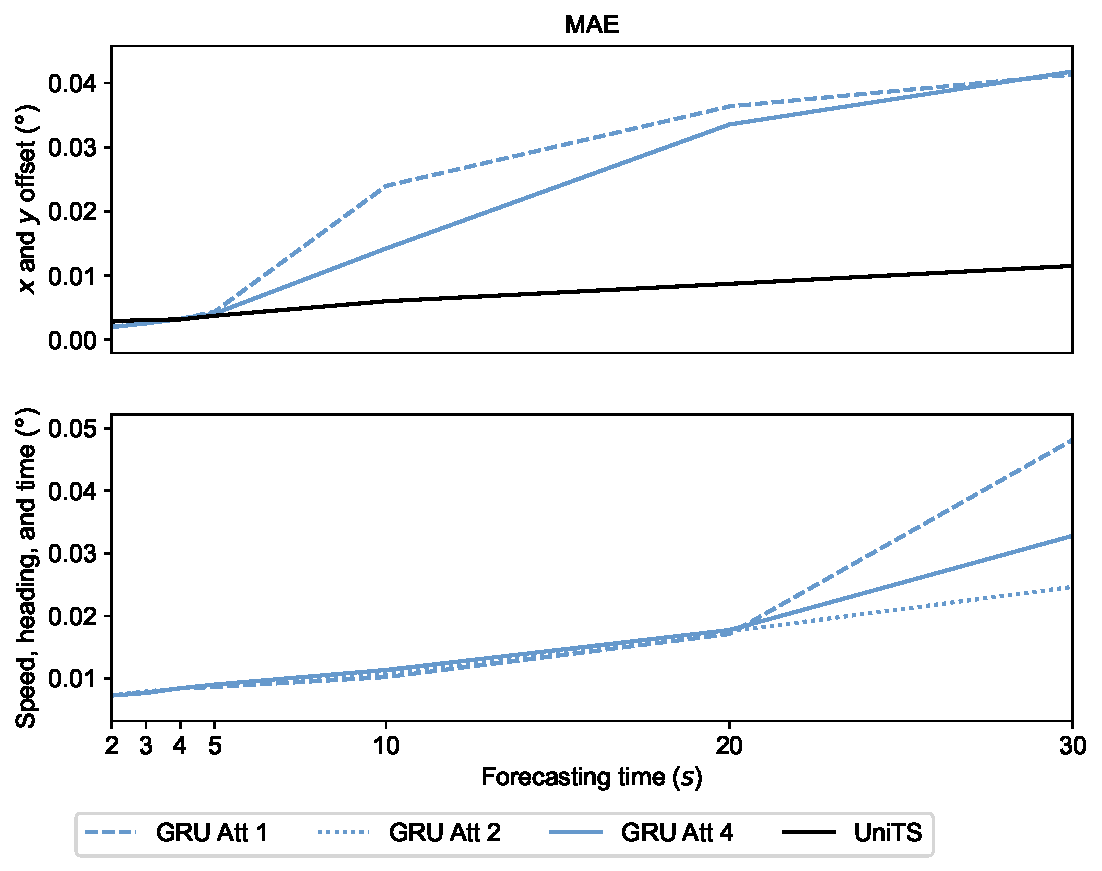
\includegraphics[width = 0.99 \linewidth]{best_MAE_traj_val.pdf}
	\caption{The average MAE across k-fold testing datasets using different trajectory estimation methods, validation datasets for all trajectories estimated in nested k-fold cross-validation by different trajectory estimation methods, RNN models, and forecasting times.}
	\label{fig:best_MAE_traj_val}
\end{figure}

The average MAE in $\degree$ ($\times 10^{-3}$), with standard deviation in brackets, across k-fold validation datasets for the trajectories in the k-fold testing datasets estimated using $x$ and $y$ offset, different RNN models, and forecasting times is listed in Table~\ref{tab:best_no_abs_MAE}.

\begin{table}[!ht]
	\centering
	\resizebox{\linewidth}{!}{
		\begin{tabular}{|c|c|c|c|c|c|c|c|}
			\hline
			Model & $2$ $s$ & $3$ $s$ & $4$ $s$ & $5$ $s$ & $10$ $s$ & $20$ $s$ & $30$ $s$ \\ \hline
			\multirow{2}{*}{GRU Att 1} & $2.07$ & $\mathbf{2.54}$ & $3.25$ & $4.36$ & $23.98$ & $36.35$ & $41.33$ \\
			 & ($0.23$) & \textbf{(}$\mathbf{0.28}$\textbf{)} & ($0.4$) & ($0.84$) & ($5.44$) & ($9.41$) & ($7.37$) \\ \hline
			\multirow{2}{*}{GRU Att 4} & $\mathbf{1.95}$ & $2.56$ & $3.22$ & $4.08$ & $14.23$ & $33.54$ & $41.8$ \\
			 & \textbf{(}$\mathbf{0.27}$\textbf{)} & ($0.29$) & ($0.31$) & ($0.41$) & ($3.09$) & ($4.46$) & ($9.25$) \\ \hline
			\multirow{2}{*}{UniTS} & $2.83$ & $3.12$ & $\mathbf{3.17}$ & $\mathbf{3.75}$ & $\mathbf{6.0}$ & $\mathbf{8.71}$ & $\mathbf{11.51}$ \\
			 & ($2.33$) & ($2.14$) & \textbf{(}$\mathbf{0.39}$\textbf{)} & \textbf{(}$\mathbf{0.58}$\textbf{)} & \textbf{(}$\mathbf{0.65}$\textbf{)} & \textbf{(}$\mathbf{0.8}$\textbf{)} & \textbf{(}$\mathbf{1.04}$\textbf{)} \\ \hline
		\end{tabular}
	}
	\caption{The average MAE in $\degree$ ($\times 10^{-3}$), with standard deviation in brackets, across k-fold validation datasets for the trajectories in the k-fold testing datasets estimated using $x$ and $y$ offset, different RNN models, and forecasting times.}
	\label{tab:best_no_abs_MAE}
\end{table}

The GRU Att 1 model achieved the lowest MAE for trajectories estimated using $x$ and $y$ offset, and a forecasting time of $3$ $s$ with an average value and standard deviation (in brackets) that equals $2.54 \times 10^{-3}$ $\degree$ ($0.28 \times 10^{-3}$ $\degree$).

The GRU Att 1 model does not make statistically significantly different predictions for longitude than the GRU Att 3, GRU Att 4, and actual value models when estimating trajectories using $x$ and $y$ offset and a forecasting time of $3$ $s$, with $p$-values equaling $0.015$, $0.033$, and $0.095$.

The GRU Att 1 model does not make statistically significantly different predictions for latitude than the GRU Twice, LSTM Linear, LSTM Twice, and actual value models when estimating trajectories $x$ and $y$ offset, and a forecasting time of $3$ $s$, with $p$-values equaling $0.04$, $0.01$, $0.001$, and $0.003$.

The GRU Att 4 model achieved the lowest MAE for trajectories estimated using $x$ and $y$ offset, and a forecasting time of $2$ $s$ with an average value and standard deviation (in brackets) that equals $1.95 \times 10^{-3}$ $\degree$ ($0.27 \times 10^{-3}$ $\degree$).

The GRU Att 4 model does not make statistically significantly different predictions for longitude than the GRU Att 1, GRU Att 2, GRU Att 3, UniTS, and actual value models when estimating trajectories using $x$ and $y$ offset and a forecasting time of $2$ $s$, with $p$-values equaling $0.428$, $0.146$, $0.813$, $0.013$, and $0.014$.

The GRU Att 4 model does not make statistically significantly different predictions for latitude than the GRU Att 2, GRU Att 3, and UniTS models when estimating trajectories $x$ and $y$ offset, and a forecasting time of $2$ $s$, with $p$-values equaling $0.123$, $0.096$, and $0.02$.

The UniTS model achieved the lowest MAE for trajectories estimated using $x$ and $y$ offset, and a forecasting time of $4$, $5$, $10$, $20$, and $30$ $s$ with average values and standard deviation (in brackets) that equal $3.17 \times 10^{-3}$ $\degree$ ($0.39 \times 10^{-3}$ $\degree$), $3.75 \times 10^{-3}$ $\degree$ ($0.58 \times 10^{-3}$ $\degree$), $6.0 \times 10^{-3}$ $\degree$ ($0.65 \times 10^{-3}$ $\degree$), $8.71 \times 10^{-3}$ $\degree$ ($0.8 \times 10^{-3}$ $\degree$), and $11.51 \times 10^{-3}$ $\degree$ ($1.04 \times 10^{-3}$ $\degree$) respectively.

The UniTS model does not make statistically significantly different predictions for longitude than the RNN Linear model when estimating trajectories using $x$ and $y$ offset and a forecasting time of $4$ $s$, with a $p$-value equaling $0.004$.

The UniTS model does not make statistically significantly different predictions for latitude than the GRU Att 1, and LSTM Third models when estimating trajectories $x$ and $y$ offset, and a forecasting time of $4$ $s$, with $p$-values equaling $0.312$, and $0.116$.

The UniTS model does not make statistically significantly different predictions for longitude than the LSTM Twice model when estimating trajectories using $x$ and $y$ offset and a forecasting time of $10$ $s$, with a $p$-value equaling $0.276$.

The UniTS model does not make statistically significantly different predictions for latitude than the GRU Att 2, and GRU Att 3 models when estimating trajectories $x$ and $y$ offset, and a forecasting time of $10$ $s$, with $p$-values equaling $0.401$, and $0.801$.

Figure~\ref{fig:best_haversine_traj_val} contains the average haversine distance in $km$ across k-fold testing datasets using different trajectory estimation methods, validation datasets for all trajectories estimated in nested k-fold cross-validation by different trajectory estimation methods, RNN models, and forecasting times.

\begin{figure}[!ht]
	\centering
	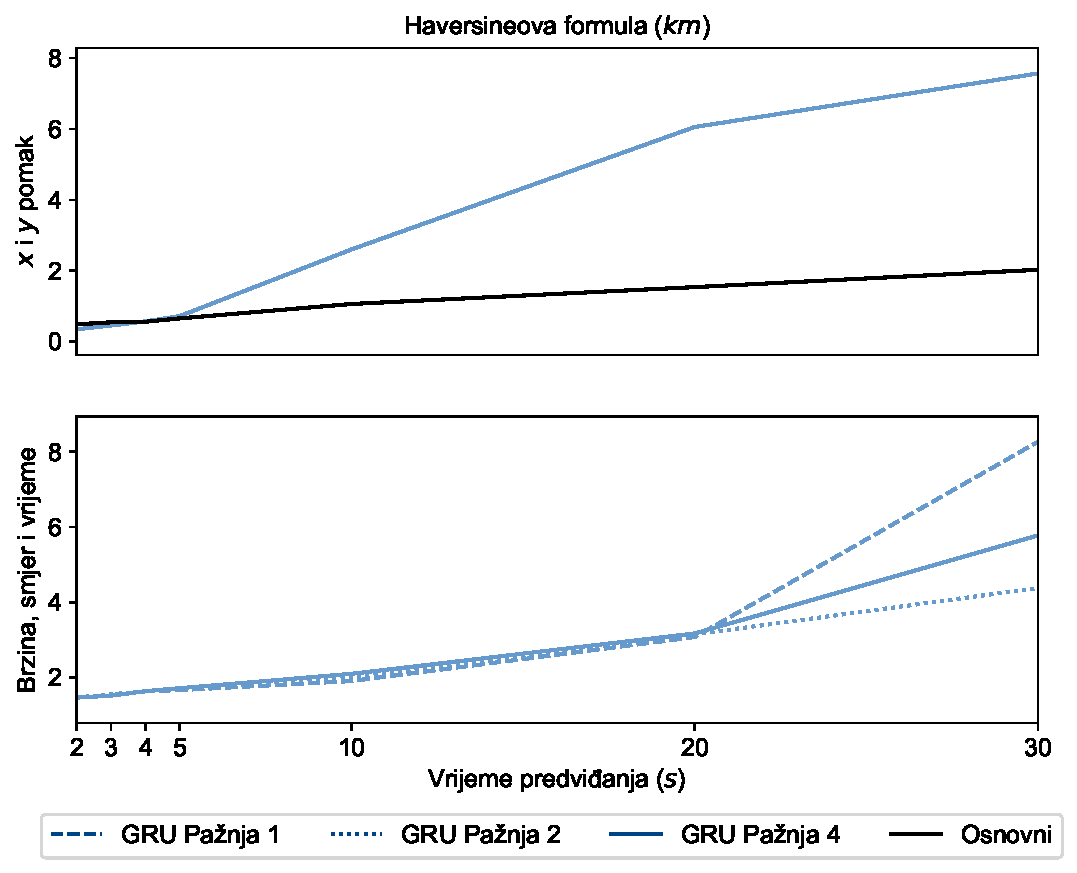
\includegraphics[width = 0.99 \linewidth]{best_haversine_traj_val.pdf}
	\caption{The average haversine distance in $km$ across k-fold testing datasets using different trajectory estimation methods, validation datasets for all trajectories estimated in nested k-fold cross-validation by different trajectory estimation methods, RNN models, and forecasting times.}
	\label{fig:best_haversine_traj_val}
\end{figure}

The average haversine distance in $km$, with standard deviation in brackets, across k-fold validation datasets for the trajectories in the k-fold testing datasets estimated using $x$ and $y$ offset, different RNN models, and forecasting times is listed in Table~\ref{tab:best_no_abs_haversine}.

\begin{table}[!ht]
	\centering
	\resizebox{\linewidth}{!}{
		\begin{tabular}{|c|c|c|c|c|c|c|c|}
			\hline
			Model & $2$ $s$ & $3$ $s$ & $4$ $s$ & $5$ $s$ & $10$ $s$ & $20$ $s$ & $30$ $s$ \\ \hline
			\multirow{2}{*}{GRU Att 4} & $\mathbf{0.346}$ & $\mathbf{0.452}$ & $0.569$ & $0.719$ & $2.599$ & $6.056$ & $7.567$ \\
			 & \textbf{(}$\mathbf{0.046}$\textbf{)} & \textbf{(}$\mathbf{0.052}$\textbf{)} & ($0.055$) & ($0.073$) & ($0.577$) & ($0.834$) & ($1.868$) \\ \hline
			\multirow{2}{*}{UniTS} & $0.485$ & $0.542$ & $\mathbf{0.558}$ & $\mathbf{0.653}$ & $\mathbf{1.059}$ & $\mathbf{1.536}$ & $\mathbf{2.025}$ \\
			 & ($0.365$) & ($0.338$) & \textbf{(}$\mathbf{0.071}$\textbf{)} & \textbf{(}$\mathbf{0.098}$\textbf{)} & \textbf{(}$\mathbf{0.124}$\textbf{)} & \textbf{(}$\mathbf{0.157}$\textbf{)} & \textbf{(}$\mathbf{0.209}$\textbf{)} \\ \hline
		\end{tabular}
	}
	\caption{The average haversine distance in $km$, with standard deviation in brackets, across k-fold validation datasets for the trajectories in the k-fold testing datasets estimated using $x$ and $y$ offset, different RNN models, and forecasting times.}
	\label{tab:best_no_abs_haversine}
\end{table}

The GRU Att 4 model achieved the lowest haversine distance for trajectories estimated using $x$ and $y$ offset, and a forecasting time of $2$, and $3$ $s$ with average values and standard deviation (in brackets) that equal $0.346$ $km$ ($0.046$ $km$), and $0.452$ $km$ ($0.052$ $km$) respectively.

The GRU Att 4 model does not make statistically significantly different predictions for longitude than the GRU Att 1, GRU Att 2, GRU Att 3, UniTS, and actual value models when estimating trajectories using $x$ and $y$ offset and a forecasting time of $2$ $s$, with $p$-values equaling $0.428$, $0.146$, $0.813$, $0.013$, and $0.014$.

The GRU Att 4 model does not make statistically significantly different predictions for latitude than the GRU Att 2, GRU Att 3, and UniTS models when estimating trajectories $x$ and $y$ offset, and a forecasting time of $2$ $s$, with $p$-values equaling $0.123$, $0.096$, and $0.02$.

The GRU Att 4 model does not make statistically significantly different predictions for longitude than the GRU Att 1, and actual value models when estimating trajectories using $x$ and $y$ offset and a forecasting time of $3$ $s$, with $p$-values equaling $0.033$, and $0.626$.

The GRU Att 4 model does not make statistically significantly different predictions for latitude than the GRU Att 2, LSTM Linear, LSTM Twice, and actual value models when estimating trajectories $x$ and $y$ offset, and a forecasting time of $3$ $s$, with $p$-values equaling $0.002$, $0.045$, $0.093$, and $0.003$.

The UniTS model achieved the lowest haversine distance for trajectories estimated using $x$ and $y$ offset, and a forecasting time of $4$, $5$, $10$, $20$, and $30$ $s$ with average values and standard deviation (in brackets) that equal $0.558$ $km$ ($0.071$ $km$), $0.653$ $km$ ($0.098$ $km$), $1.059$ $km$ ($0.124$ $km$), $1.536$ $km$ ($0.157$ $km$), and $2.025$ $km$ ($0.209$ $km$) respectively.

The UniTS model does not make statistically significantly different predictions for longitude than the RNN Linear model when estimating trajectories using $x$ and $y$ offset and a forecasting time of $4$ $s$, with a $p$-value equaling $0.004$.

The UniTS model does not make statistically significantly different predictions for latitude than the GRU Att 1, and LSTM Third models when estimating trajectories $x$ and $y$ offset, and a forecasting time of $4$ $s$, with $p$-values equaling $0.312$, and $0.116$.

The UniTS model does not make statistically significantly different predictions for longitude than the LSTM Twice model when estimating trajectories using $x$ and $y$ offset and a forecasting time of $10$ $s$, with a $p$-value equaling $0.276$.

The UniTS model does not make statistically significantly different predictions for latitude than the GRU Att 2, and GRU Att 3 models when estimating trajectories $x$ and $y$ offset, and a forecasting time of $10$ $s$, with $p$-values equaling $0.401$, and $0.801$.

